Con riferimento al precedente esercizio, tabulare il massimo errore di approssimazione (calcolato come sopra indicato), sia utilizzando le ascisse equidistanti
che quelle di Chebyshev su menzionate, relativo alla spline cubica naturale interpolante $f(x)$ su tali ascisse.

\hspace*{\fill}
\par\noindent\rule{\textwidth}{0.4pt}
\hspace*{\fill}

\begin{lstlisting}[language=Matlab, caption=Codice Matlab]
f = @(x) 1 ./ (1 + x.^2);
a = -5;
b = 5;
n = 2 : 2 : 40;
x = linspace(a, b, 10001)';
fx = f(x);
ex = zeros(length(n), 1); ec = zeros(length(n), 1);

ax1 = subplot(2, 1, 1);
for i = 1 : length(n)
	xi = linspace(a, b, n(i) + 1)';
	fxi = f(xi);
	yxi = spline3(xi, fxi, x);
	plot(ax1, x, yxi)
	hold on
	ex(i) = norm(fx - yxi, inf);
end
legend('2', '4', '6', '8', '10', '12', '14', '16', '18', '20', '22', '24', '26', '28', '30', '32', '34', '36', '38', '40')
hold off

ax2 = subplot(2, 1, 2);
for i = 1 : length(n)
	ci = ceby(n(i) + 1, a, b);
	x = linspace(min(ci), max(ci), 10001)';
	fx = f(x);
	fci = f(ci);
	yci = spline3(ci, fci, x);
	plot(ax2, x, yci)
	hold on
	ec(i) = norm(fx - yci, inf);
end
legend('2', '4', '6', '8', '10', '12', '14', '16', '18', '20', '22', '24', '26', '28', '30', '32', '34', '36', '38', '40')
hold off
\end{lstlisting}

Le seguenti figure mostrano la spline cubica naturale interpolante $f(x)$, al variare del numero di ascisse di interpolazione ($=3,5,7,9...41$), utilizzando ascisse equidistanti e ascisse di Chebyshev:
\begin{figure}[H]
	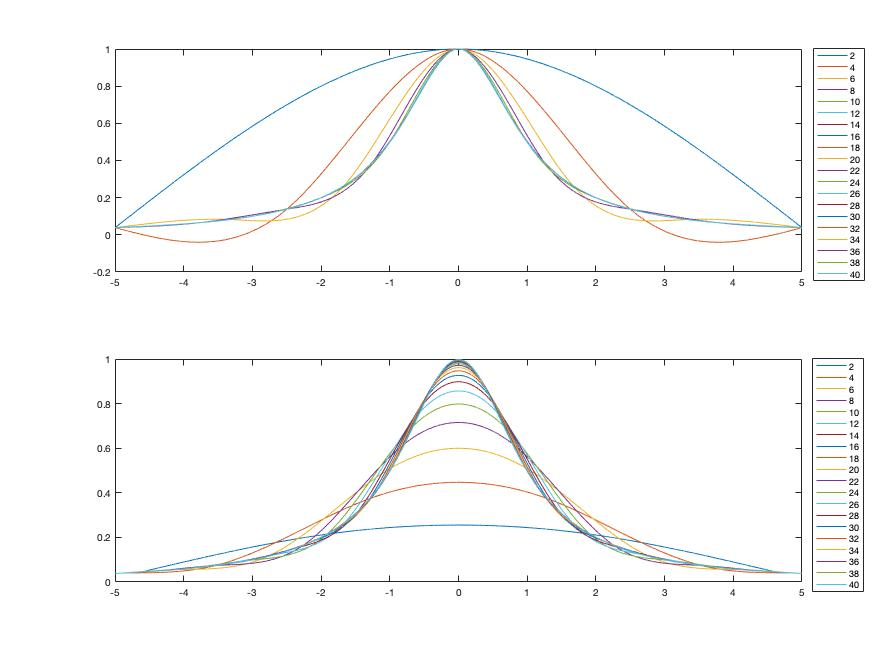
\includegraphics[width=\textwidth]{Chapter-4/Exercise-20/plot.jpg}
	\caption*{Spline cubica naturale con n° di ascisse $[3,5,7,9,..,41]$, interpolante ascisse equidistanti e di Chebyshev, rispettivamente}
\end{figure}

Nelle seguenti tabelle è riportato come varia il massimo errore di approssimazione, al variare del numero di ascisse di interpolazione:\\\
\begin{table}[H]
	\begin{minipage}{0.5\textwidth}
		\centering
		\caption{Massimo errore con ascisse equispaziate}
		\begin{tabular}{|c|c|}
			\hline
			$n$ & $Errore$ \\
			\hline
			$2$  & $6.011945468114989e-01$ \\ 
			$4$  & $2.793134075196790e-01$ \\ 
			$6$  & $1.293000883540983e-01$ \\ 
			$8$  & $5.607385287856159e-02$ \\ 
			$10$ & $2.197382574958184e-02$ \\ 
			$12$ & $6.908801437725876e-03$ \\ 
			$14$ & $2.482863475717023e-03$ \\ 
			$16$ & $3.745402833395861e-03$ \\ 
			$18$ & $3.717998718041349e-03$ \\ 
			$20$ & $3.182857643173609e-03$ \\ 
			$22$ & $2.529653088972128e-03$ \\ 
			$24$ & $1.925792361618828e-03$ \\ 
			$26$ & $1.427047863662545e-03$ \\ 
			$28$ & $1.039053280856961e-03$ \\ 
			$30$ & $8.243623332672145e-04$ \\ 
			$32$ & $6.554986812412622e-04$ \\ 
			$34$ & $5.237082286350114e-04$ \\ 
			$36$ & $4.210035707792326e-04$ \\ 
			$38$ & $3.408377962142994e-04$ \\ 
			$40$ & $2.779765405962475e-04$ \\ 
			\hline
		\end{tabular}
	\end{minipage}
	\hspace*{\fill}
	\begin{minipage}{0.5\textwidth}
		\centering
		\caption{Massimo errore con ascisse di Chebyshev}
		\begin{tabular}{|c|c|}
			\hline
			$n$ & $Errore$ \\
			\hline
			$2$  & $7.446676877937543e-01$ \\ 
			$4$  & $5.529300734832576e-01$ \\ 
			$6$  & $4.003323237631188e-01$ \\ 
			$8$  & $2.848203213309948e-01$ \\ 
			$10$ & $2.017549216803890e-01$ \\ 
			$12$ & $1.432128531581862e-01$ \\ 
			$14$ & $1.022002088148625e-01$ \\ 
			$16$ & $7.343428357692028e-02$ \\ 
			$18$ & $5.316898347940879e-02$ \\ 
			$20$ & $3.880700384549352e-02$ \\ 
			$22$ & $2.856026101132547e-02$ \\ 
			$24$ & $2.119758438849628e-02$ \\ 
			$26$ & $1.586841915298964e-02$ \\ 
			$28$ & $1.198228990567030e-02$ \\ 
			$30$ & $9.126979380553069e-03$ \\ 
			$32$ & $7.013001529651786e-03$ \\ 
			$34$ & $5.435813807564749e-03$ \\ 
			$36$ & $4.249991716239854e-03$ \\ 
			$38$ & $3.351491356512803e-03$ \\ 
			$40$ & $2.665402637469283e-03$ \\ 
			\hline
		\end{tabular}
	\end{minipage}
\end{table}

Dunque, possiamo notare che il \textbf{fenomeno di Runge} non è più presente, dato che l'errore di approssimazione non tende più a infinito. Questo risultato è dato
dall'utilizzo delle spline come metodo di interpolazione, grazie alle quali è possibile suddividere la partizione dei nodi in più parti, calcolando su
ciascun sottointervallo un polinomio interpolante di grado non elevato (in questo caso di grado 3, dato che abbiamo utilizzato una spline cubica).
